\chapter{Propiedades magnéticas de la materia}
\chaptermark{Propiedades magnéticas materia}

\begin{miparrafo}
	En ausencia de un campo magnético la mayor parte de la materia no manifiesta propiedades magnéticas; eso es debido a que internamente, los campos magnéticos generados por el movimiento de los electrones están compensados unos con otros. Sin embargo al someter a un material, sea el que sea, a la acción de un campo magnético exterior, se produce una distorsión del movimiento electrónico lo que provoca la aparición de un momento magnético opuesto al campo exterior. Además, se da el caso de materiales que poseen de antemano un momento magnético y al ser sometidos a la acción del campo se produce una alineación de dichos momentos, lo que favorece la propagación del campo magnético.
\end{miparrafo}


\section[Comportamiento de la materia en un campo magnético: paramagnetismo, diamagnetismo, ferromagnetismo]{Comportamiento de la materia en un campo magnético: paramagnetismo, diamagnetismo, ferromagnetismo\sectionmark{Para, diam y ferro - magnetismo}}
\sectionmark{Para, diam y ferro - magnetismo}


\begin{multicols}{2}
Consideremos un campo magnético creado por un solenoide. Introducimos una muestra con un poco de material sujeta por un dinamómetro en el interior de solenoide y apreciamos que aparece una fuerza que, curiosamente, no es más intensa en el centro del solenoide sino en sus bordes, donde el campo magnético es menor:
$\ \displaystyle \pdv{B}{z}$ es mayor en el borde que en el centro.

$B_{centro}=\dfrac{nI\mu_0}{L}$ 

$B_{bordes}=\dfrac 1 2 \dfrac{nI\mu_0}{L}$
\begin{figure}[H]
	\centering
	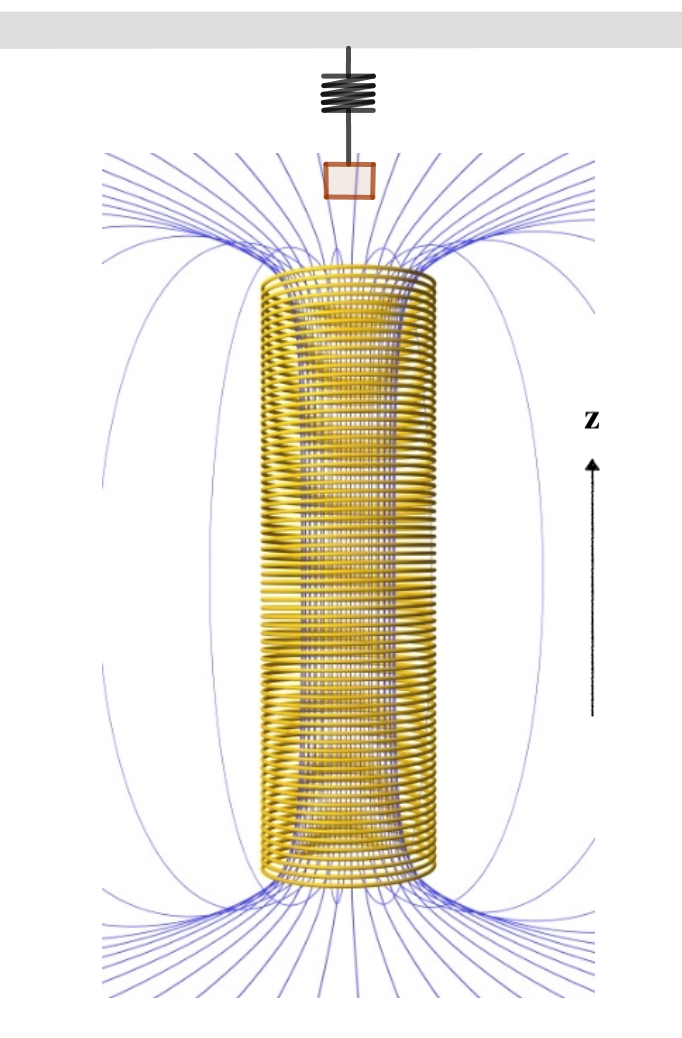
\includegraphics[width=0.45\textwidth]{imagenes/imagenes28/T28IM01.png}
\end{figure}	
\end{multicols}

Haremos una gran gama de experiencias como esta variando el material. La muestra debe ser pequeña.

Se observa:

\begin{itemize}
\item Experimentalmente se pone de manifiesto que la fuerza es directamente proporcional a la masa e independiente de su forma geométrica.
\item Algunas sustancias son atraídas hacia abajo, donde el campo magnético crece; otras son repelidas hacia arriba, donde el campo decrece. Y esto ocurre con independencia de la orientación del campo magnético (sentido de la corriente).	
\end{itemize}

Elegiremos el signo $-$ hacia arriba, hacia donde el campo decrece y $+$ hacia abajo, donde crece el campo.

La fuerza sobre $1 \ \mathrm{g}$ de nuestra muestra en un campo magnético con $B_z=1.8\times 10^4\ \mathrm{Gaus}$ y $\displaystyle \pdv {B_z} {z}=1.7\times 10^3 \ \mathrm{G\ cm}^{-2}$, a $21\ ^o$ es:



\begin{table}[H]
\centering
\begin{tabular}{lllll}
\multicolumn{1}{l|}{\textit{Sustancia}} & \textit{Fuerza(dinas)} & \textit{$\quad$} & \multicolumn{1}{l|}{\textit{Sustancia}} & \textit{Fuerza(dinas)} \\
\multicolumn{2}{c}{\textbf{Diamagnéticas}}                       &                  & \multicolumn{2}{c}{\textbf{Paramagnéticas}}                      \\ \cline{1-2} \cline{4-5} 
\multicolumn{1}{l|}{$H_2O$}             & $-22$                  &                  & \multicolumn{1}{l|}{$Na$}               &                        \\
\multicolumn{1}{l|}{$Cu$}               & $-2.6$                 &                  & \multicolumn{1}{l|}{$Al$}               &                        \\
\multicolumn{1}{l|}{$Pb$}               & $-3.7$                 &                  & \multicolumn{1}{l|}{$Cl_2Cu$}           &                        \\
\multicolumn{1}{l|}{$ClNa$}             & $-15$                  &                  & \multicolumn{1}{l|}{$SO_4Ni$}           &                        \\
\multicolumn{1}{l|}{$SiO_2$}            & $-16$                  &                  & \multicolumn{1}{l|}{$O_2\ (liq)$}       &                        \\
\multicolumn{1}{l|}{$C$, diamante}      & $-16$                  &                  & \multicolumn{2}{c}{\textbf{Ferromagnéticas}}                     \\ \cline{4-5} 
\multicolumn{1}{l|}{$C$, grafito}       & $-110$                 &                  & \multicolumn{1}{l|}{$Fe$}               & +400000                \\
\multicolumn{1}{l|}{$N_2\ (liq)$}       & $-10 \ (78 K)$         &                  & \multicolumn{1}{l|}{$F_e3O_4$}          & +120000               
\end{tabular}
\end{table}

Por definición, las sustancias que reaccionan hacia arriba se llaman \emph{\textbf{diamagnéticas}}, a las que lo hacen hacia abajo se les llama \emph{\textbf{paramagnéticas}}. En este tipo de sustancias, el efecto aumenta al aumentar la temperatura (\emph{Ley de Curie}). Cuando la fuerza es elevada, las sustancias se llaman 
\emph{\textbf{ferromagnéticas}}.


El $Na$ es paramagnético, pero el $ClNa$ es diamagnético. En cambio, el $Cu$ es diamagnético y el $Cl_2Cu$ es paramagnético.

Hay una cosa que tienen en común las sustancias paramagnéticas y diamagnéticas que las diferencia de las ferromagnéticas: imaginemos que disminuimos a la mitad el valor de la intensidad de la corriente que circula por el solenoide, el valor del campo magnético también disminuirá a la mitad. Se observa que tanto las sustancias paramagnéticas como las diamagnéticas reaccionan con una fuerza que es la cuarta parte del valor absoluto encontrado antes de disminuir la corriente mientras que las sustancias ferromagnéticas reaccionan con una fuerza reducida solo a la mitad, en consecuencia:

$$F_{\text{Dia y Para-magnéticas}} \propto I^2; \qquad F_{\text{Ferromagnéticas}} \propto I$$

Esto es lo que hay que explicar teóricamente.

\section[Fuerzas en un dipolo magnético en un campo externo]{Fuerzas en un dipolo magnético en un campo externo\sectionmark{Fuerza en dipolo magnético}}

\sectionmark{Fuerza en dipolo magnético}

Siguiendo la idea de Ampère, suponemos la materia sometida a prueba constituida por corrientes moleculares que dan lugar un momento dipolar.


\begin{multicols}{2}
El circuito representa la corriente molecular. Supongamos que está contenido en el plano $XY$

En cada elemento del circuito, ley de Ampère:

$\dd \vec F = I \dd \vec l \times \vec B=$

$=I\vec \dd l \times (\vec u_r B_r + \vec k B_z)=$

$=I\dd \vec l \times \vec u_r B_r + I\dd \vec l \times \vec k B_z$
\begin{figure}[H]
	\centering
	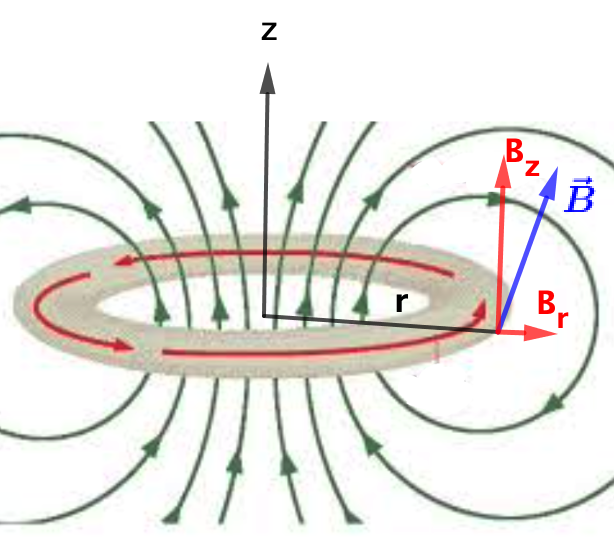
\includegraphics[width=0.45\textwidth]{imagenes/imagenes28/T28IM02.png}
\end{figure}	
\end{multicols}
El primer término lleva el sentido de $-\vec k$ y el segundo término el de $\vec u_r$, por lo que éste último término no contribuirá a la fuerza total.

Para toda la espira, integrando:

$\displaystyle F=\oint_C I\dd l B_r = I 2\pi r B_r$

Veamos si podemos expresar $I$ en función del gradiente $\displaystyle \pdv{B_z}{z}$. Para ello usaremos el th. de Gauss para el campo magnético, $\displaystyle \oint_S \vec B \cdot \dd \vec S=0$

\begin{multicols}{2}
Suponemos, $z\to B_z;$

$ z+\dd z \to B_z+\dd B_z$

$B_z+\dd B_z=\displaystyle B_z+ \pdv{B_z}{z}\dd z$

Calculamos el flujo:
\begin{figure}[H]
	\centering
	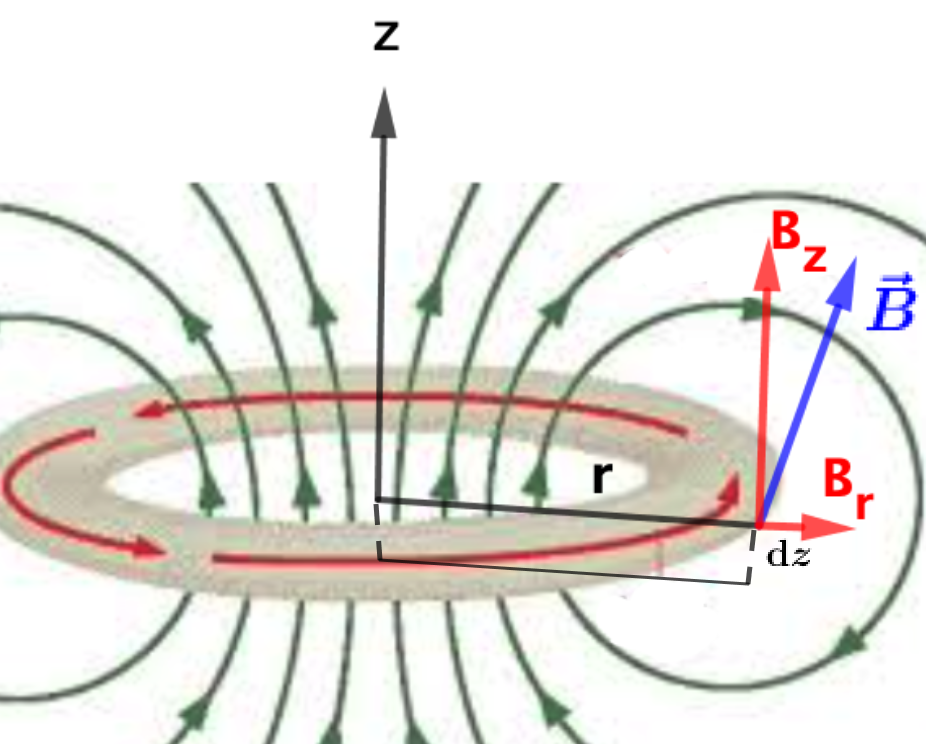
\includegraphics[width=0.3\textwidth]{imagenes/imagenes28/T28IM03.png}
\end{figure}	
\end{multicols}

Flujo = Flujo que entra por abajo + flujo que sale por arriba + flujo que sale por la superficie lateral:

$\displaystyle -B_z \pi r^2 + \left( B_z+ \pdv{B_z}{z} \right) \pi r^2 + 2\pi r \dd z B_r = 0$

De aquí, se obtiene: $\ B_r=-\dfrac r 2 \displaystyle \pdv{B_z}{z}$, por lo que

$$F \ = \ -I\pi r^2 \displaystyle \pdv{B_z}{z} \ = \ -m\pdv{B_z}{z}$$

\section{Explicación clásica del magnetismo}


Imaginemos un campo como el del solenoide tal que al aumentar $z$, $B_z$ disminuye. Esto es debido al signo menos del gradiente.

Como $\vec m$ es un vector y $\displaystyle \pdv{B_z}{z}$ hace referencia al la componente vectorial del campo, se obtiene:

$$\vec B \uparrow \ \downarrow \vec m \ \to \ F \ \uparrow ;\qquad 
  \vec B \uparrow \ \uparrow \vec m \ \to \ F \ \downarrow$$

Si el momento dipolar magnético $\vec m$ asociado a una espira está asociado a la dirección paralela de un campo magnético $\to$ la fuerza que actúa sobre el dipolo va en el sentido en el cual la intensidad del campo es creciente. Si $\vec m$ es antiparalelo al campo externo $\to$ la fuerza actúa en el sentido de la intensidad del campo decreciente.

si $\displaystyle \pdv{B_z}{z}=0 \ \to \ F=0$, si no hay gradiente, variación del campo $\to$ no hay fuerza.

\begin{miparrafodestacado}
	El quid de la cuestión estriba en el por qué un material tiene un momento magnético que se orienta paralelamente al campo magnético externo para reaccionar paramagnéticamente o se orienta antiparalelamente al campo para reaccionar diamagnéticamente.
	
	Además, cuando la $I$ se reduce a la mitad, las sustancias para y diamagnéticas ven el efecto reducido a la cuarta parte mientras que en las ferromagnéticas solo se reduce a la mitad.
\end{miparrafodestacado}

Tendremos que exigir que $\ m \propto I;\ \displaystyle \pdv{B_z}{z} \propto I \ \to \ F \propto I^2$, para sustancias para o diamagnéticas.

Para ferromagnéticas, habrá de ocurrir que $\ m $ independiente de $I$ , $\ \ \displaystyle \pdv{B_z}{z} \propto I \ \to \ F \propto I$

\textbf{Problemas que se plantean:}

\begin{itemize}
	\item ?`Por qué unas sustancias tienen $\vec m$  paralelo o antiparalelo a $\vec B$?
	\item ?`Por qué el momento dipolar magnético $m$ de las sustancias para o diamagnéticas ha de ser proporcional a $B$ (o a $I$) mientras que en las sustancias ferromagnéticas ha de ser independiente del mismo?
\end{itemize}

\textcolor{gris}{Para explicar bien el electromagnétisno es necesaria la mecánica cuántica.}

\section{Teoría del diamagnetismo}

$\vec m = -\dfrac{e}{2m_e} \ \vec L;\qquad \vec L= I_{nercia}\  \vec \omega = m_er^2 \ \vec \omega \quad \to \quad \vec m=-\dfrac 1 2 e r^2 \ \vec \omega$

Tenemos las dos posibles situaciones para cualquier electrón en su órbita:

\begin{figure}[H]
	\centering
	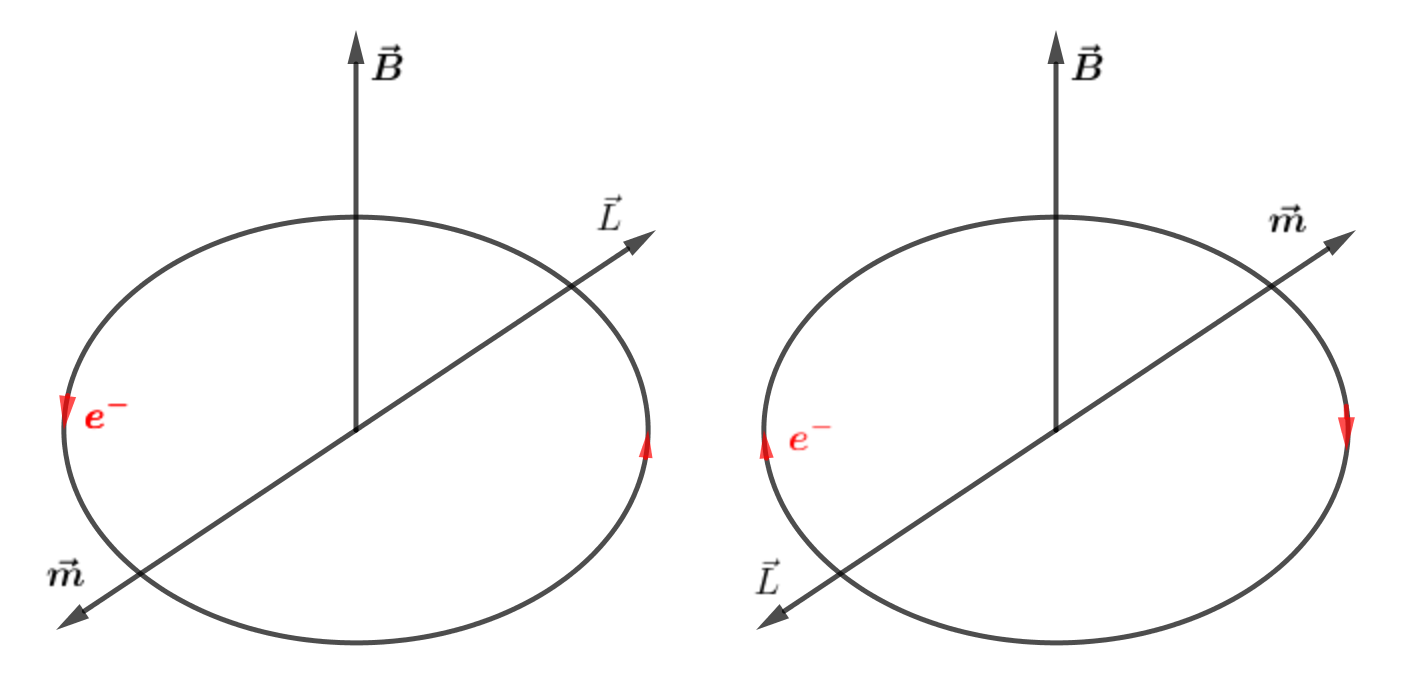
\includegraphics[width=0.75\textwidth]{imagenes/imagenes28/T28IM04.png}
\end{figure}

Estudiemos como influye el campo magnético externo sobre el movimiento de los electrones alrededor del núcleo.

$\vec M=\vec m \times \vec B$; $\ \displaystyle \dv{\vec L}{t}= \vec m\times \vec B=-\dfrac{e}{2m_e}\vec L \times \vec B$

Tanto para en un caso u otro el sentido de rotación del extremos de $\vec L$ es el mismo, sentido contrario a las agujas del reloj.

\begin{figure}[H]
	\centering
	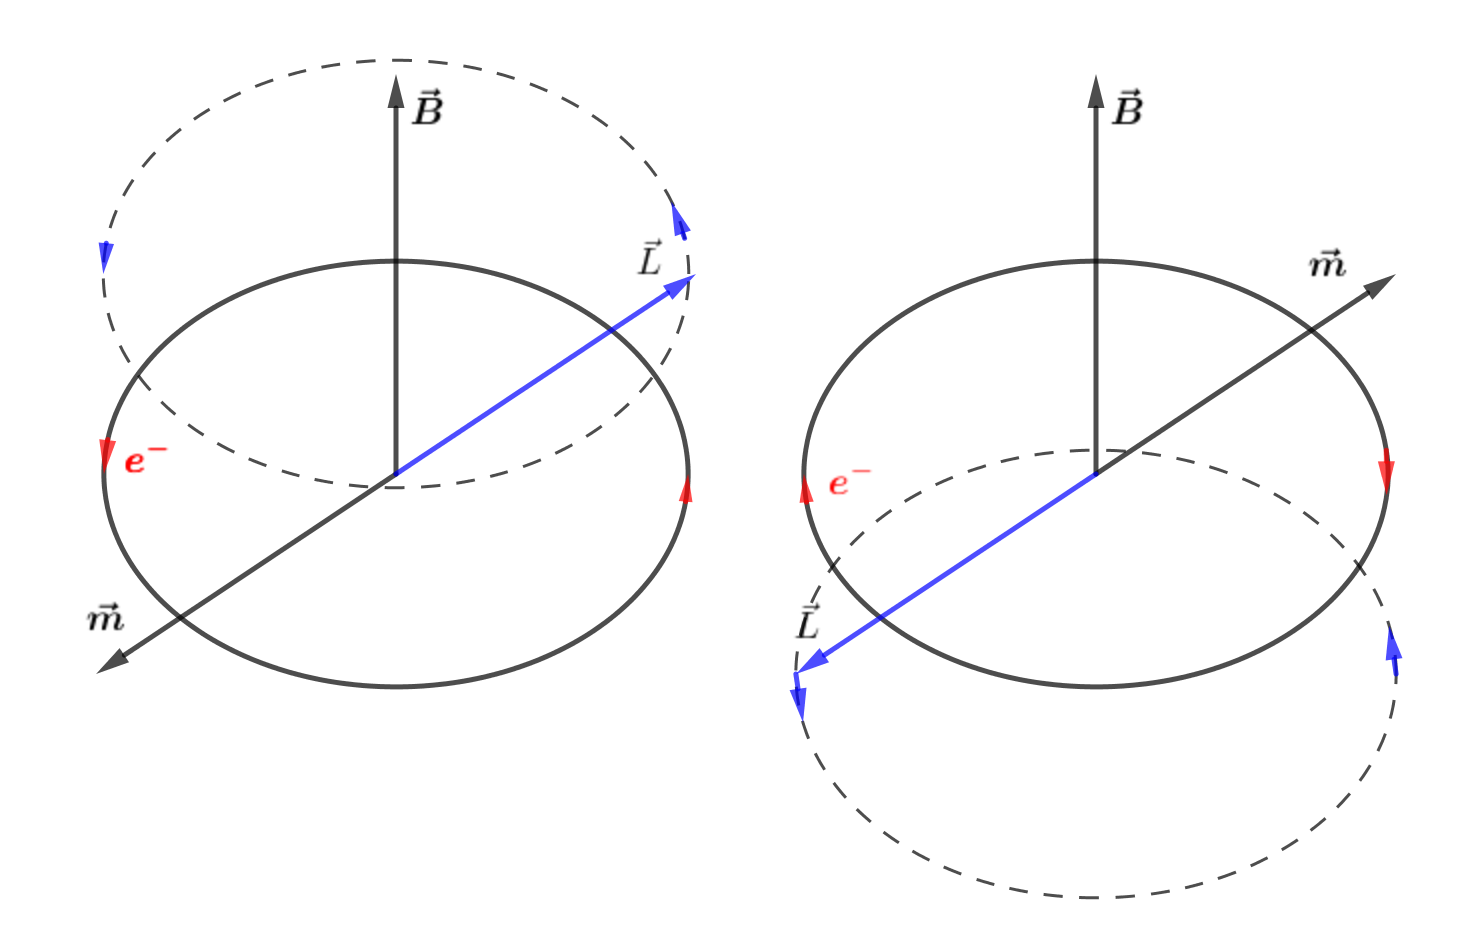
\includegraphics[width=0.75\textwidth]{imagenes/imagenes28/T28IM05.png}
\end{figure}

\begin{multicols}{2}
\emph{arco = ángulo $\times$ radio}

$\dd L= L \sin \varphi \dd \theta$

$\dd \vec L = - \vec L \times \dfrac{\vec B}{B} \ \dd \theta$

$\displaystyle \dv{\vec L}{t}=-\vec L \times  \dfrac{\vec B}{B} \ \dv{\theta}{t}= - \vec L \times  \dfrac{\vec B}{B} \ \Omega$
\begin{figure}[H]
	\centering
	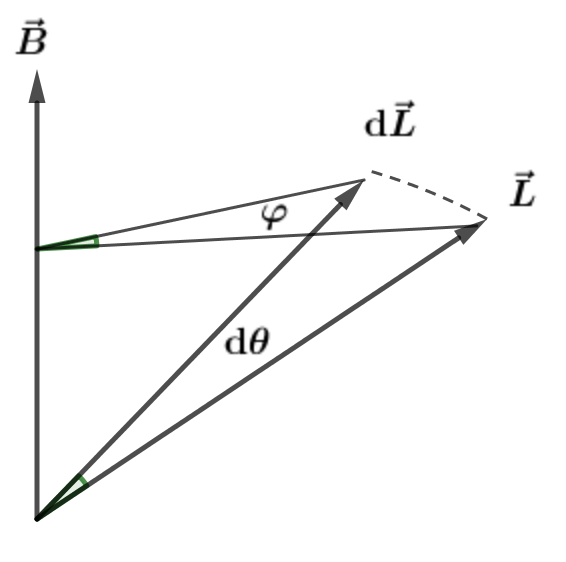
\includegraphics[width=0.3\textwidth]{imagenes/imagenes28/T28IM06.png}
\end{figure}	
\end{multicols}

Comparando con el resultado anterior, $\ \Omega=-\dfrac{eB}{2m_e}$, en forma vectorial:

$\vec \Omega \ = \ \dfrac{e\ \vec B}{2m_e}\ $  representa una \emph{precesión} de la órbita del electrón.

Así, el movimiento del electrón se deberá a dos causas: un movimiento electrostático respecto al núcleo, $\vec \omega$ y el debido al campo magnético externo, $\vec \Omega$. Finalmente, $\vec \omega_T=\vec \omega+\vec \Omega$

Aparece un momento dipolar inducido por la presencia de $\Omega$, que llamaremos $\vec m_{ind}$ que será:

$$m_{ind} \ = \ -\dfrac 1 2 e r^2 \ \vec \Omega \ =\ - \dfrac 1 4 \dfrac {e^2\ r^2}{m_e}\ \vec B$$

Cualquier electrón, en presencia de un campo magnético externos, tendrá un momento dipolar que será suma del que tenía más el inducido.

Por término medio y desde el punto de vista clásico, todos los sentidos de giros posibles se van a cancelar pero los momentos dipolares inducidos no se cancelan nunca por tener siempre la misma dirección y el mismo sentido (contrario a las agujas del reloj).

$\vec m_{total}=\sum \vec m_{ind} \neq 0$, todos tienen la misma dirección y sentido.

$$ \vec m \ = \ - \dfrac 1 4 \dfrac {e^2\ r^2}{m_e}\ \vec B$$

la fuerza se dirige hacia donde la intensidad del campo magnético crece.

Según este resultado, todas las sustancias deberían ser diamagnéticas. \emph{?`Dónde están las paramagnéticas?}

Efectivamente, todas las ustancias tienen una componente diamagnética, pero en las  paramagnéticas ha de ocurrir algo que haga aparecer otro momento dipolar magnético orientado en el mismo sentido del campo magnético externo. \textbf{\emph{Hasta aquí llega el electromagnetismo clásico.}}

Vamos a usar una mecánica clasico-cuántica.

$\text{electrones en átonos } \to 
	\begin{cases}
		\text{número par } &\to  \text{\ diamagnéticas} \\ 
		\text{número impar } &\to  \text{\ paramagnéticas}
 	\end{cases}$

En las sustancias diamagnéticas, el único momento dipolar que se manifiesta es el inducido. En las sustancias paramagnéticas aparece un nuevo momento dipolar magnético. La naturaleza solo presenta una excepción a esta regla, el $Cu^{29}$ que con número impar de electrones se comporta como diamagnético.

\begin{miparrafodestacado}
	\textbf{Conclusiones}: \emph{Todos los átomos de la naturaleza, en principio, tienen caracter diamagnético. Aquellos con número par de electrones cancelan dos a dos sus momentos dipolares y se comportan diamagnéticamente. En las sustancias con número impar de electrones (excepto el $Cu^{29}$) tienen un momento dipolar que no se cancela y supera al $\vec m_{ind}$ por lo que son paramagnéticas. }
\end{miparrafodestacado}

\subsection{Cálculo de la susceptibilidad diamagnética}

Vector magnetización $\ \vec M=n\vec m=\chi_m \vec H$, $n$ número de átomos, $\chi_m$ susceptibilidad magnética.

$\mu'=\dfrac{\mu}{\mu_0}=1+\chi_m$. $\mu'$ permeabilidad relativa.

En las sustancias diamagnéticas, $\vec M$ antiparalelo a $\vec H$ (o $\vec B$), para esas sustancias $\chi_m<0$ y $\mu'<1$

Para sustancias paramagnéticas, $\vec M$ paralelo $\vec H$, por lo que $\chi:m>0$ y $\mu'>1$, es decir $\mu>\mu_0$

En las sustancias ferromagnéticas, también ocurre que $\vec M$ paralelo a $\vec H$, pero $\chi_m>>0 \ \to \mu' >> 1 \ \to \ \mu >>\mu_0$

Como $\vec M=\chi_m \vec H$ y $\vec m_{imd}=-\dfrac 1 4 \dfrac{e^2r^2}{m_e}\vec B$, entonces:

$\vec M_{\text{diamagnético}}= n\  \vec m_{ind} = - \dfrac 1 4 \dfrac{e^2r^2n}{m_e} \ \vec B=- \dfrac 1 4 \dfrac{e^2r^2n}{m_e} \ \mu_o \vec H=\chi_m \ \vec H$

$$\chi_m \ = \ -\dfrac 1 4 \ \dfrac{e^2\ r^2\ n}{m_e} \ \mu_0$$

\section{Teoría del paramagnetismo}

El paramagnetismo solo se manifiesta en átomos con número impar de electrones (excepto el $Cu^{29}$). Sometemos una muestra de un material paramagnético, de número impar de electrones, a la acción de un campo magnético externo, $\vec B$. Para cada uno de estos átomos, 

$\mathcal E_p=-\vec m \cdot \vec B=-mB\cos \varphi$, donde $\varphi$ es el ángulo entre $\vec m$ y $\vec B$

Un resultado de \emph{mecánica estadística} asegura quepara ua muestra con $\mathcal E_4$, se cumple:
$\ \displaystyle \dv{n(\varphi)}{\Omega}=n_0\ e^{-\mathcal E_p / KT}; \quad n(\varphi)=\dv{m}{\tau}.\ $ Donde, $n(\varphi)$ es el número de elementos por unidad de volumen orientados en la dirección $\varphi$; $K=R/N_A$ es la constante de Boltzman, $1.3805\times 10^{-23}\ \mathrm{J\ K}^{-1}$, y $T$ es la temperatura absoluta.

En el caso del dipolo magnético, $\ \displaystyle \dv{n(\varphi)}{\Omega}= n_0\ e^{mB\cos \varphi / KT}$

Aproximando, $\ \dfrac{mB\cos \varphi}{KT} \sim \dfrac{10^{-23}\times 2 \times 0.5}{1.4\times 10^{-23} \times 300} \sim 0.002$, o sea, el argumento de la exponencial es del orden de milésimas.

Desarrollo en serie McLaurin: $\ e^x=1+x+\dfrac{x^2}{2!}¡\dfrac{x^3}{3!}+\cdots$, quedándonos a primer orden (despreciamos billonésimas frente a milésimas,

$$\displaystyle \dv{n(\varphi)}{\Omega} \ \approx \ n_0 \left[ 1 + \dfrac {mB\cos \varphi}{KT} \right]$$

$ \text{Para } \vec B \ \uparrow \uparrow \ \vec m \ \to \  \varphi=0 \ \to \ \cos \varphi = 1 \\
\text{Para } \vec B \ \uparrow \downarrow \ \vec m \ \to \  \varphi=\pi \ \to \ \cos \varphi = -1 $

Despejando e integrando, obtenemos el número de dipolos por unidad de volumen en la dirección $\varphi$

$\displaystyle \int \dd n(\varphi) \ = \ n_0\ \int \left[ 1 + \dfrac {mB\cos \varphi}{KT} \right] \ \dd \Omega$

$\displaystyle M=\int_0^n  m \cos \varphi \dd n(\varphi) \ = \ \int_\Omega m \cos \varphi \left[ 1 + \dfrac {mB\cos \varphi}{KT} \right] \ \dd \Omega$

En el caso axial, $\ \dd \Omega = 2\pi \sin \varphi \dd \varphi = -2\pi \dd (\cos \varphi) \ \Rightarrow $

$ M=\dfrac{nm^2B}{3KT}\ , \qquad \text{con } n_0=n/4\pi$

Como $M=\chi_m H=\chi_m \dfrac B {\mu_0}$, finalmente

$$\chi_m \ = \ \dfrac {n\ m^2 \ \mu_0}{K \ \ T}$$

Esta es la demostración de \emph{Lancevin}. Hemos obtenido una \textbf{susceptibilidad paramagnética} positiva, con $\vec m \ || \ \vec B$ y que es inversamente proporcional a la temperatura absoluta, $\chi_m \propto \dfrac 1 T$ para materiales paramagnéticos, como establece la ley experimental de \emph{Pierre Curie}.

\section[Ferromagnetismo, ferrimagnetismo y antiferromagnetismo]{Ferromagnetismo, ferrimagnetismo y antiferromagnetismo\sectionmark{Ferro, ferri y antiferro - magnetismo}}
\sectionmark{Ferro, ferri y antiferro - magnetismo}

\begin{footnotesize}

El ferromagnetismo es un fenómeno físico en el que se produce ordenamiento magnético de todos los momentos magnéticos de una muestra, en la misma dirección y sentido. La interacción magnética que hace que los polos magnéticos tiendan a disponerse en la misma dirección y sentido ha de extenderse por todo el sólido para alcanzar el ferromagnetismo.

Los ferromagnetos están divididos en dominios magnéticos, separados por superficies conocidas como paredes de Bloch. En cada uno de estos dominios, todos los momentos magnéticos están alineados. 

Al someter un material ferromagnético a un campo magnético intenso, los dominios tienden a alinearse con este, de forma que aquellos dominios en los que los dipolos están orientados con el mismo sentido y dirección que el campo magnético inductor aumentan su tamaño. Este aumento de tamaño se explica por las características de las paredes de Bloch, que avanzan en dirección a los dominios cuya dirección de los dipolos no coincide; dando lugar a un monodominio. Al eliminar el campo, el dominio permanece durante cierto tiempo.

\begin{figure}[H]
	\centering
	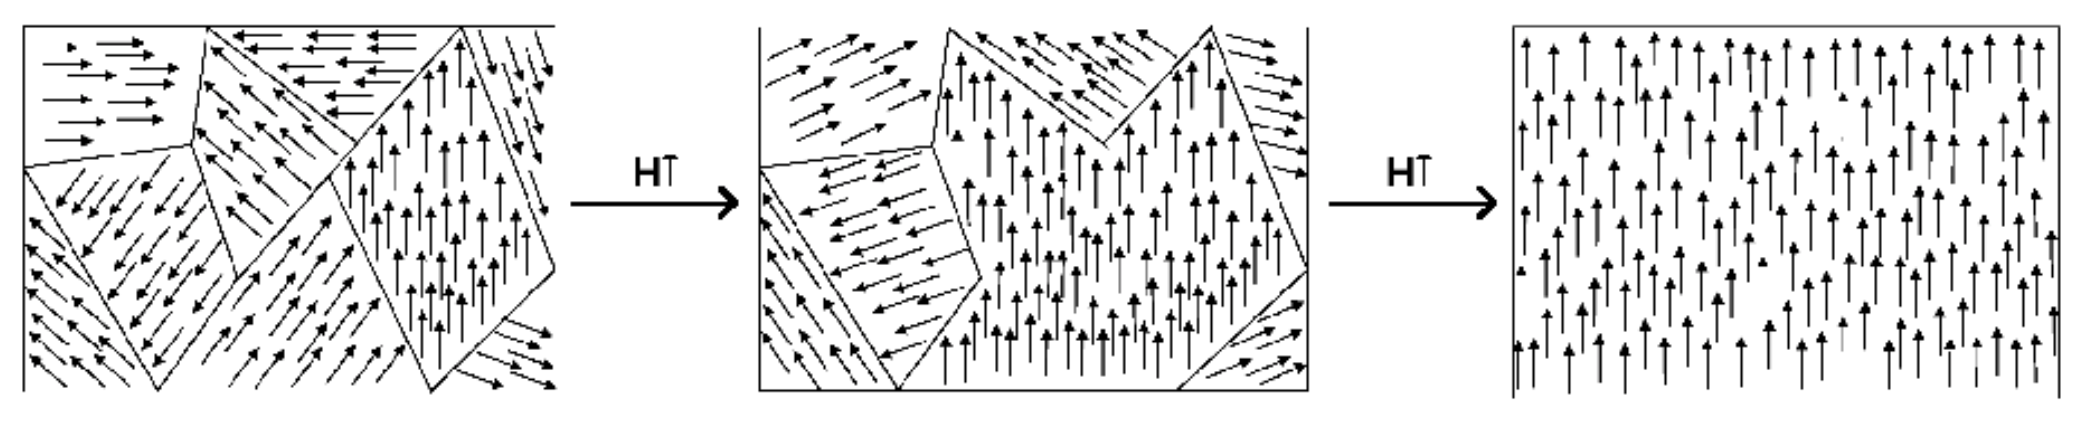
\includegraphics[width=1\textwidth]{imagenes/imagenes28/T28IM07.png}
\end{figure}


El ferrimagnetismo es un fenómeno físico en el que se produce ordenamiento magnético de los momentos magnéticos de una muestra de modo que todos los momentos magnéticos están alineados en la misma dirección pero no en el mismo sentido. Así que algunos de ellos están opuestos y se anulan entre sí, en parte o completamente. Sin embargo estos momentos magnéticos que se pueden anular están distribuidos aleatoriamente y no consiguen anular por completo la magnetización espontánea. Un ferrimagneto es una muestra de material que presenta ferrimagnetismo. 

El ferrimagnetismo también presenta, como el ferromagnetismo, magnetizaciones permanentes y de saturación (punto en el que ya no aumenta la magnetización por más que aumentemos la fuerza del campo). Otra similitud es que por encima de la temperatura de Curie se pierde el ferrimagnetismo y el material pasa a ser paramagnético.

Los materiales ferrimagnéticos proceden normalmente de la ferrita. Las ferritas, siendo materiales cerámicos, son buenos aislantes eléctricos. 

El antiferromagnetismo es el ordenamiento magnético de todos los momentos magnéticos de una muestra, durante la aplicación de un campo magnético, en la misma dirección. Al cesar el campo magnético externo la mitad de los momentos magnéticos de la muestra cambian en sentido inverso (por pares, por ejemplo, o una subred frente a otra). La interacción antiferromagnética, interacción magnética que hace que los momentos magnéticos tiendan a disponerse en la misma dirección y en sentido inverso, cancelándolos si tienen el mismo valor absoluto, o reduciéndolos si son distintos, ha de extenderse por todo un sólido para alcanzar el antiferromagnetismo.

Como el ferromagnetismo, la interacción antiferromagnética se destruye a alta temperatura. La temperatura por encima de la cual no se aprecia el antiferromagnetismo se llama temperatura de Neel, nombrada en honor del químico francés  Louis Néel (1904 – 2000), que había identificado por primera vez este tipo de ordenamiento magnético. Por encima de esta, los compuestos son típicamente paramagnéticos.

Generalmente, los antiferromagnetos están divididos en dominios magnéticos. En cada uno de estos dominios, todos los momentos magnéticos están alineados. En las fronteras entre dominios hay cierta energía potencial.

Al someter un material antiferromagnético a un campo magnético intenso, algunos de los momentos magnéticos se alinean paralelamente con él, aun a costa de alinearse también paralelo a sus vecinos (superando la interacción antiferromagnética). Generalmente, se requiere un campo magnético muy intenso para conseguir alinear todos los momentos magnéticos de la muestra.


\begin{figure}[H]
	\centering
	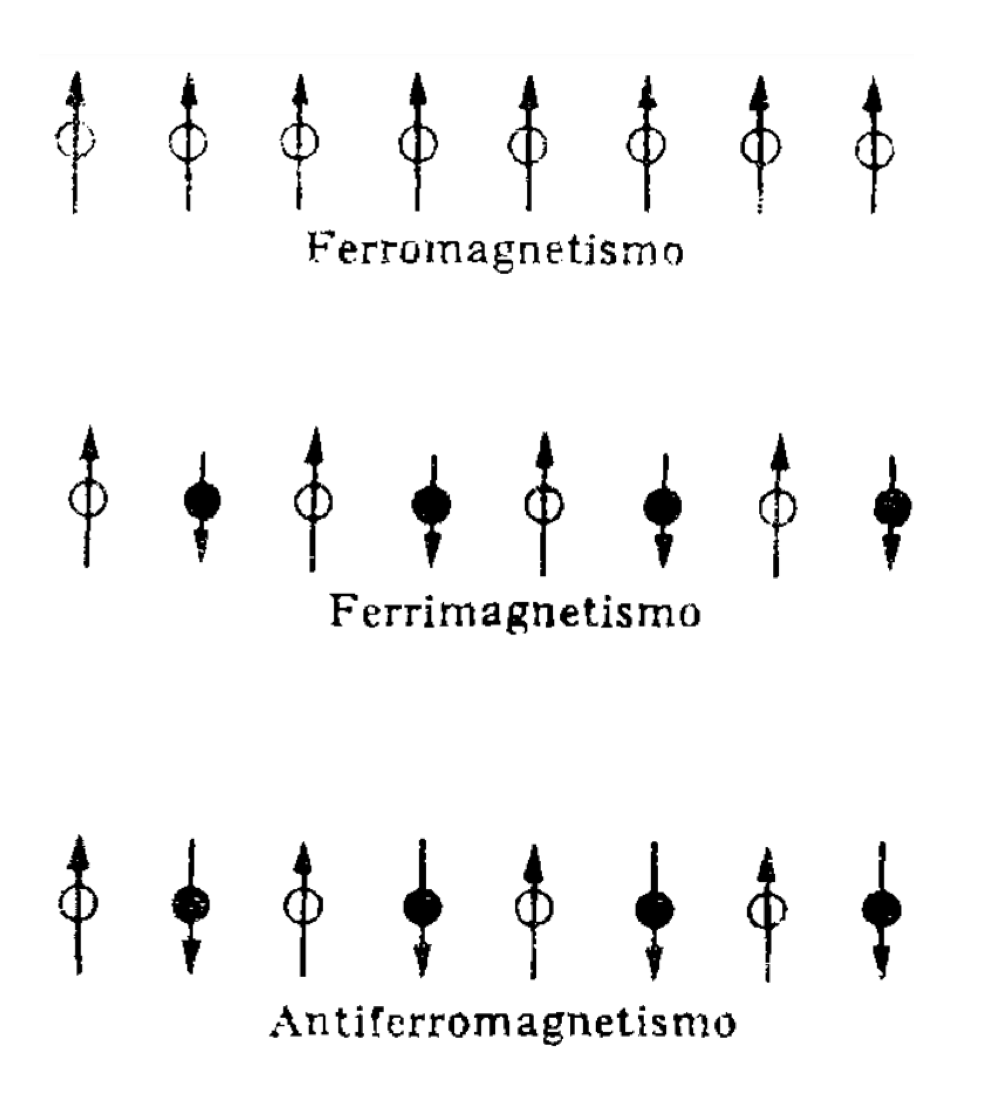
\includegraphics[width=.6\textwidth]{imagenes/imagenes28/T28IM08.png}
\end{figure}

\end{footnotesize}


\newpage %***********************************************
\begin{myblock}{Electromagnetismo}
En este capítulo hemos discutido los campos eléctrico y magnético estáticos como dos entidades separadas, sin relación alguna entre ellas, excepto que las fuentes del campo eléctrico son las cargas eléctricas y las del campo magnético son las corrientes eléctricas. En consecuencia hemos obtenido dos conjuntos de ecuaciones separadas, las cuales aparecen en la tabla en ambas formas, integral y diferencial. 

\begin{table}[H]
\centering
\begin{tabular}{l|l|l}
\multicolumn{1}{c|}{\textbf{Ley}}        & \multicolumn{1}{c|}{\textbf{Forma integral}}                                     & \multicolumn{1}{c}{\textbf{Forma diferencial}}                                       \\ \hline
Ley de Gauss para \\ el campo eléctrico  & $\quad \displaystyle \oint_S \vec E \cdot \dd \vec S = \dfrac{q}{\varepsilon_0}$  & $\quad \overrightarrow{\nabla}\cdot \overrightarrow{E}=\dfrac {\rho}{\varepsilon_0}$ \\
Ley de Gauss para \\  el campo magnético  & $\quad \displaystyle \oint_S \vec B \cdot \dd \vec S = 0$                        & $\quad \overrightarrow{\nabla}\cdot \overrightarrow{B}=0$                            \\
Circulación del \\ campo eléctrico        & $\quad \displaystyle \int_L \vec E \cdot \dd \vec l = 0$                         & $\quad \overrightarrow{\nabla}\times \overrightarrow{E}=0$                           \\
Circulación del \\ campo magnético        & $\quad \displaystyle \int_L \vec B \cdot \dd \vec l = \mu_0\ I$                  & $\quad \overrightarrow{\nabla}\times \overrightarrow{B}=\mu_0 \vec J$               
\end{tabular}
\end{table}

Estas ecuaciones permiten calcular el campo eléctrico $\vec E$ y el campo magnético $\vec B$ si se conocen las cargas y las corrientes, y recíprocamente. De este modo parece como si los campos eléctrico y magnético se pudieran considerar como dos campos independientes. Sin embargo esto no es cierto, según las transformaciones de Lorentz (relatividad especial), dos observadores en movimiento relativo observan que $\vec E$ y $\vec B$.



Hemos estudiado los campos eléctrico y magnético estáticos, es decir, independientes de tiempo. En los casos que los campos dependan del tiempo, las ecuaciones precedentes requerirán algunas modificaciones. 

Todo ello formará parte de cursos superiores de \emph{electromagnetismo.}
	
\end{myblock}
